\documentclass[11pt, aspectratio=169]{beamer}

% --- Core Packages for Modern Documents ---
\usepackage{fontspec}      
\usepackage{unicode-math}
% \usepackage{xeCJK}         
% \usepackage{tipa}
\usepackage{graphicx}      
\usepackage{minted}
\usepackage{setspace}
\usepackage{kotex}
\usepackage{tikz}
\usepackage{multicol}
\usepackage{hyperref}
\usepackage{emoji}

\usetikzlibrary{
    shapes.geometric, % 다양한 도형 사용
    arrows.meta,      % 화살표 스타일 설정
    positioning       % 노드 위치 선정
}

% \xeCJKsetup{CJKspace=true}

% --- Font Setup ---
\setsansfont{Noto Sans KR} %Noto Sans KR
\setmainfont{Noto Serif KR}
\setmonofont{D2Coding}

\setmainhangulfont{Noto Sans KR}
\setsanshangulfont{Noto Serif KR}
\setmonohangulfont{D2Coding}

% \setCJKsansfont{Noto Sans KR}  %나눔바른고딕 옛한글
% \setCJKmainfont{Noto Serif KR}
% \setCJKmonofont{D2Coding}

\setmathfont{Latin Modern Math}

\newfontfamily{\tnrfont}{Times New Roman}
\newcommand{\texttnr}[1]{{\tnrfont #1}}
\newfontfamily{\ipafont}{Doulos SIL}
\newcommand{\textds}[1]{{\ipafont #1}}
\newfontfamily{\chinesefont}{Noto Sans SC}
\newcommand{\textzh}[1]{{\chinesefont #1}}

\mode<presentation>
{
  \usetheme{default}      % or try Darmstadt, Madrid, Warsaw, Marburg...
  \usecolortheme{dove} % or try albatross, beaver, crane, dove...
  \usefonttheme{default}  % or try serif, structurebold, ...
  \setbeamertemplate{navigation symbols}{}
  \setbeamertemplate{caption}[numbered]
} 

\AtBeginSection[]{
  \begin{frame}
    \vfill % Vertically center the title
    \centering
      \usebeamerfont{title}\insertsectionhead\par
    \vfill
  \end{frame}
}

\renewcommand{\arraystretch}{1.3} % Set row height for ALL tables in the document to 1.5x

\definecolor{Highlight}{HTML}{FFF2CC} % A soft yellow

\definecolor{MonokaiBackground}{HTML}{272822}
\definecolor{blocktitle}{HTML}{7A8B5D}
\definecolor{blockbody}{HTML}{F0E085}
\definecolor{normaltext}{HTML}{E5E8D5}
\definecolor{structure_color}{HTML}{D1E1E8}

\setbeamercolor{normal text}{bg=normaltext, fg=black}
\setbeamercolor{structure}{bg=structure_color, fg=black}

\setbeamercolor{block title}{bg=blocktitle, fg=white}
\setbeamercolor{block body}{bg=blockbody, fg=black}
\setbeamertemplate{footline}{
  \hfill % Pushes the content to the right
  \usebeamercolor{page number in head/foot}
  \usebeamerfont{page number in head/foot}
  \insertframenumber{} / \inserttotalframenumber
  \hspace*{2ex} % Adds a little padding from the right edge
}

\setminted{
    style=default, % dracula, native, monokai...
    linenos,       % Show line numbers
    frame=lines,   % Draw a thin frame around the code
    framesep=2mm,
    xleftmargin=6pt,
    breaklines=true
}

% 제목 정보
\title{언어의 이해}
\subtitle{3강. 언어의 소리 체계와 음운론}
\author{김미경}
\date{2025.9.17}

\begin{document}

% 제목 슬라이드
\frame{\titlepage}

% 목차
\begin{frame}[t]{목차}
\tableofcontents
\end{frame}

\section{개별 언어의 말소리 규칙}

\begin{frame}[t]{개별 언어의 말소리 목록}
    \begin{block}{음성 인벤토리}
        언어별로 사용되는 말소리의 목록
    \end{block}
    \begin{columns}
        \begin{column}[T]{0.42\textwidth}
            \begin{block}{한국어}
                \begin{tabular}{llll}
                    ㄱ & \textds{[k]}(가) & \textds{[k̚]}(박) & \textds{[g]}(아가) \\
                    ㅂ & \textds{[p]}(바) & \textds{[p̚]}(갑) & \textds{[b]}(아비) \\
                    ㅋ & \textds{[kʰ]}(카) & & \\
                    ... & & & \\
                \end{tabular}                            
            \end{block}
        \end{column}
        \begin{column}[T]{0.51\textwidth}
            \begin{block}{영어}
                \begin{tabular}{llll}
                    k & \textds{[k]}(skip) & \textds{[kʰ]}(keep) & \textds{[k’]}(수의적) \\
                    p & \textds{[p]}(spot) & \textds{[pʰ]}(pot) & \textds{[p̚]}(수의적)\\
                    ... & & & \\
                \end{tabular}                            
            \end{block}
        \end{column}
    \end{columns}
\end{frame}

\begin{frame}[t]{개별 언어 말소리의 결합}
    \begin{block}{말소리 결합의 순서 제약}
        개별 언어의 말소리가 한 단위를 만들 때 결합하는 순서에는 제약이 있음
    \end{block}
    \begin{block}{{한국어 \textds{[m]}, \textds{[u]}, \textds{[n]}의 결합}}
        \begin{itemize}
            \item 가능: \textds{[mun]}, \textds{[num]}
            \item 불가능: \textds{[mnu]}, \textds{[nmu]}, \textds{[umn]}, \textds{[unm]}
        \end{itemize}        
    \end{block}
    \begin{block}{{영어 어두 \textds{[b]}, \textds{[r]}의 결합}}
        \begin{itemize}
            \item 가능: \textds{[br]} (‘brick’, ‘bring’...)
            \item 불가능: \textds{[rb]}
        \end{itemize}
    \end{block}    
\end{frame}

\begin{frame}[t]{개별 언어 말소리의 결합}
    \begin{block}{말소리 결합의 위치 제약}
        개별 언어의 말소리가 한 단위를 만들 때에는 출현하는 위치에 제약이 있음
    \end{block}
    \begin{block}{한국어 \textds{[ŋ]}}
        \begin{itemize}
            \item 어두에서 허용되지 않음
        \end{itemize}
    \end{block}
    \begin{block}{한국어 \textds{[ɾ]}}
        \begin{itemize}
            \item 기본: 어두에서 허용되지 않음 (내방\textsuperscript{4}(來訪)) vs. 왕래(往來))
            \item 외래어: 어두에서도 허용됨 (라면, 라디오, 렌즈, 라부부, ... )
        \end{itemize}
    \end{block}
\end{frame}

\begin{frame}[t]{개별 언어 말소리의 결합}
    \begin{block}{말소리 결합의 종류 제약}
        개별 언어의 말소리가 결합해서 만드는 한 단위의 종류에는 제약이 있음
    \end{block}
    \begin{block}{한국어}
        \begin{itemize}
            \item 가능: CV(\textds{[ka]}), VC(\textds{[ak]}), CVC(\textds{[kak]}), V(\textds{[a]})
            \item 불가능: C(\textds{[k]}), CCV(\textds{[kka]}), CCCV(\textds{[kkka]}), VCC(\textds{[akk]}), VCCC(\textds{[akkk]}), CC(\textds{[kk]}), ...
        \end{itemize}
    \end{block}
    \begin{block}{한국어 패턴의 일반화}
        \begin{itemize}
            \item 모음이 1개 있어야 함
            \item 앞뒤에 자음이 1개까지 올 수 있음
        \end{itemize}
    \end{block}
\end{frame}

\begin{frame}[t]{개별 언어 말소리의 결합}
    \begin{block}{말소리 결합의 종류 제약}
        개별 언어의 말소리가 결합해서 만드는 한 단위의 종류에는 제약이 있음
    \end{block}
    \begin{block}{영어}
        V(a), VC(at), VCC(ask), VCCC(asked), CV(no), CVC(not), CVCC(ramp), CVCCC(ramps), CCV(flew), CCVC(flute), CCVCC(flutes), CCVCCC(crafts), CCCV(spree), CCCVC(spleen), CCCVCC(strength), CCCVCCC(strengths)
    \end{block}
    \begin{block}{영어 패턴의 일반화}
        \begin{itemize}
            \item 모음이 1개 있어야 함
            \item 앞뒤에 자음이 3개까지 올 수 있음
        \end{itemize}
    \end{block}
\end{frame}

\begin{frame}[t]{개별 언어 말소리 규칙에 어긋나는 소리의 발음}
    \begin{columns}
        \begin{column}{0.46\textwidth}
            \begin{block}{유사한 소리로 바꾸기}
                \begin{itemize}
                    \item \texttnr{Nguyễn} \rightarrow 영어 Nguyen \textds{[nuˈjɛn]}
                    \item bye \rightarrow 한국어 바이 \textds{[pai]}
                \end{itemize}
            \end{block}            
        \end{column}
        \begin{column}{0.47\textwidth}
            \begin{block}{다른 소리 끼워넣기}
                \begin{itemize}
                    \item \texttnr{Nguyễn} \rightarrow 한국어 응우옌 \textds{[ɯŋujen]}
                    \item strike \rightarrow 한국어 스트라이크
                \end{itemize}
            \end{block}            
        \end{column}
    \end{columns}
    \begin{block}{무시하기}
        \begin{itemize}
            \item 아랍어의 \textds{[ʔ]}를 발음하지 않음
            \item \texttnr{Nguyễn} \rightarrow 영어 Nguyen \textds{[wɪn]}
            \item Ptolemaîos \rightarrow 영어 Ptolemy \textds{[ˈtɒləmi]}
        \end{itemize}
    \end{block}
    \emoji{television} \href{https://youtu.be/d_JBDM6IC20?t=37}{\underline{프랑스계 성씨 ‘Poilievre’ \textds{[pwa.ljɛvʁ]}를 캐나다 영어로 발음하기}}\\
    {\scriptsize “...And so in France, they tend to roll the last R: Poilievre. But no one says it that way here, so Poly-ev is fine. I mean, I’m easy with first name basis. At the end of the day, Brian, I don’t care how you say my name, as long as you know how to put an X beside it on election day”}
\end{frame}

\section{음성과 음운}

\begin{frame}[t]{개별 언어의 말소리 체계}
    \begin{block}{음성(phone)}
        \begin{itemize}
            \item 사람이 발음 기관을 사용해서 만들어내는 분절음과 초분절음
            \item \textds{[ ]} 기호로 감싸서 표기
            \item 개별 언어별로 주로 사용되는 음성들이 정해져 있음
            \item 개별언어에서 사용되지 않는 음성을 개인이 사용하면 낯설게 들림
        \end{itemize}
    \end{block}
    \begin{itemize}
        \item ‘매일두유’: 한국어 화자의 발음 vs. 외국어 화자의 발음
        \item ‘즨짜’: \emoji{television} \href{https://youtu.be/FB6jrxNt6Qk}{\underline{고의로 발음 낯설게 하기}}
        \item 랩 흉내: \emoji{television}\href{https://youtu.be/AMiApAli848}{\underline{고의로 억양 낯설게 하기}}
    \end{itemize}
\end{frame}

\begin{frame}[t]{개별 언어의 말소리 체계}
    \begin{block}{음운}
        \begin{itemize}
            \item 한 언어 사용자가 서로 구분된다고 인지하는 분절음과 초분절음
            \item / / 기호로 감싸서 표기
        \end{itemize}
    \end{block}
    \textbf{‘구분된다’} \rightarrow 대립성과 변별성이 있다
    \begin{columns}
        \begin{column}[T]{0.46\textwidth}
            \begin{block}{음소(phoneme)}
                화자들이 서로 구분된다고 인지하는 분절음
            \end{block}            
            \begin{itemize}
                \item 영어 pet \textds{/pet/} vs. bet \textds{/bet/}
                \item 한국어 풀 \textds{/pʰul/} vs. 불 \textds{/pul/} 
            \end{itemize}            
        \end{column}
        \begin{column}[T]{0.47\textwidth}
            \begin{block}{운소}
                화자들이 서로 구분된다고 인지하는 초분절음
            \end{block}            
            \emoji{television} \href{https://youtube.com/watch?v=GwGDfwgiOn4}{\underline{한국어 동남방언 ‘2의 e승’}}
        \end{column}
    \end{columns}
\end{frame}

\begin{frame}[t]{음소와 변이음}
    \begin{block}{1:1 또는 1:多}
        \begin{itemize}
            \item 하나의 음소는 하나 이상의 음성을 실현형으로 가질 수 있음    
            \item 음소와 음성의 연결은 언어마다 다름
        \end{itemize}
    \end{block}
    \begin{columns}
        \begin{column}[T]{0.46\textwidth}
            한국어 \textds{/p/}
                \begin{itemize}
                    \item 밥 \textds{/pap/} \textds{[pap]}
                    \item 밥을 \textds{/papɯl/} \textds{[pabɯl]}
                \end{itemize}
            한국어 \textds{/pʰ/}
            \begin{itemize}
                \item 팝 \textds{/pʰap/} \textds{[pʰap]}
            \end{itemize}
        \end{column}
        \begin{column}[T]{0.47\textwidth}
            미국 영어 \textds{/p/} 
            \begin{itemize}
                \item pie \textds{/paɪ/} \textds{[pʰaɪ]}
                \item spy \textds{/spaɪ/} \textds{[spaɪ]}
            \end{itemize}
            미국 영어 \textds{/b/} 
            \begin{itemize}
                \item bye \textds{/baɪ/} \textds{[baɪ]}
            \end{itemize}
        \end{column}
    \end{columns}
   \begin{block}{변이음(allophone)}
        음소와 1:多 관계에 있는 음성이 개별 언어의 말소리 지식 내에서 갖는 지위
    \end{block}
\end{frame}

\begin{frame}[t]{음소와 변이음}
    \begin{block}{음소 추출하기}
        \begin{itemize}
            \item 한 언어에서 최소대립쌍을 성립시키는 분절음
            \item 최소대립쌍의 차이를 이루는 각각의 소리들을 서로 다른 음소로 간주
        \end{itemize}
    \end{block}
    \begin{block}{최소대립쌍(minimal pair)}
        하나의 소리만 다르고 나머지 모든 소리는 같은, 서로 다른 단어의 쌍
    \end{block}
    한국어
    \begin{itemize}
        \item 발 : 팔 \rightarrow \textds{/p/}와 \textds{/pʰ/}는 각각 한국어의 음소
        \item 등 : 든 \rightarrow \textds{/ŋ/}와 \textds{/n/}은 각각 한국어의 음소
        \item 다 : 두 : 도 \rightarrow \textds{/a/}, \textds{/u/}, \textds{/o/}는 각각 한국어의 음소
    \end{itemize}
\end{frame}

\begin{frame}[t]{음소와 변이음}
    서로 다른 음성이 확인되는데 최소대립쌍을 찾을 수 없다면?
    \begin{block}{변이음 추출하기}
        \begin{itemize}
            \item 한 언어에서 상보적 분포를 이루고, 최소대립쌍을 성립시키지 않는 분절음들
            \item 동일한 음소의 변이음으로 간주
        \end{itemize}
    \end{block}
    \begin{block}{상보적 분포}
        서로 다른 두 음성이 각각 나타나는 환경이 중복되지 않는 관계
    \end{block}
    한국어
    \begin{itemize}
        \item \textds{[b]}: 모음과 유성음 사이에서 출현
        \item \textds{[p]}: 그 외의 모든 환경에서 출현
    \end{itemize}
\end{frame}

\begin{frame}[t]{음소와 변이음}
    \begin{block}{변이음 중에서 대표 표기 고르기}
        \begin{itemize}
            \item 실제로 관찰되는 것: 변이음들
            \item 변이음들을 포괄하는 추상적인 음소를 설정
            \item 이 때, 가장 출현 환경에 제약이 적은 변이음의 기호를 음소 기호로 고름
        \end{itemize}
    \end{block}
    미국 영어 \textds{[t], [tʰ], [ʔ], [ɾ]}\\
    \begin{tabular}{|l|l|l|l|l|}
        \hline
        \textbf{변이음} & \textbf{출현 환경} & \textbf{단어} & \textbf{음소 층위} & \textbf{음성 층위} \\
        \hline
        \textds{[t]} & \textcolor{red}{그 외 대부분의 환경에서 출현} & star & \textds{/stɑːʳ/} & \textds{[stɑːʳ]}\\
        \textds{[tʰ]} & 어두에서 출현 & teacher & \textds{/tiːtʃəʳ/} & \textds{[tʰiːtʃəʳ]} \\
        \textds{[ʔ]} & 어말 또는 성절음 \textds{/n̩/} 앞에서 출현 & button & \textds{/bʌtn̩/} & \textds{[bʌʔn̩]} \\
        \textds{[ɾ]} & 모음 사이에서 출현 & butter & \textds{/bʌtəʳ/} & \textds{[bʌɾəʳ]}\\
        \hline
    \end{tabular}
    \\
    \rightarrow 미국 영어에 \textds{/t/} 음소를 설정
\end{frame}

\begin{frame}[t]{음소와 변이음: 연습}
    다음 단어 목록이 영어의 \textds{[p]}와 \textds{[pʰ]}가 출현할 수 있는 모든 경우의 수라고 가정할 때, 영어의 \textds{[p]}와 \textds{[pʰ]}가 서로 다른 음소인지, 한 음소의 변이음인지 판단하세요.
    \begin{itemize}
        \item spat \textds{[spæt]} 
        \item spool \textds{[spul]} 
        \item speak \textds{[spik]} 
        \item pat \textds{[pʰæt]} 
        \item pool \textds{[pʰul]} 
        \item peek \textds{[pʰik]}
    \end{itemize}
\end{frame}

\begin{frame}[t]{자유 변이(free variation)}
    서로 다른 음성이 확인되는데, 최소대립쌍을 찾을 수 없고, 상보적 분포도 이루지 않는다면?
    \begin{block}{자유 변이}
        음소가 단어의 의미를 바꾸지 않으면서 다른 음성으로 실현되는 경우
    \end{block}
    \begin{itemize}
        \item 영어의 수의적 방출음 \textds{[k’]} (anarchic \textds{[ænɑːʳkɪk]}) vs. \textds{[ænɑːʳk’ɪk]})
        \item 영어의 수의적 어말 파열음 \textds{[p̚]} (leap \textds{[lip]} vs. \textds{[lip̚]})
    \end{itemize}
    \begin{columns}
        \begin{column}{0.46\textwidth}
            \begin{block}{자유 변이 vs. 음소}
                \begin{itemize}
                    \item 둘 다 동일한 환경에서 출현 가능
                    \item 최소대립쌍 성립 여부가 다름
                \end{itemize}
            \end{block}
        \end{column}
        \begin{column}{0.47\textwidth}
            \begin{block}{자유 변이 vs. 변이음}
                \begin{itemize}
                    \item 둘 다 최소대립쌍을 성립시키지 않음
                    \item 상보적 분포 성립 여부가 다름
                \end{itemize}
            \end{block}
        \end{column}
    \end{columns}
\end{frame}

\begin{frame}[t]{{한국어의 음소: 자음, 반모음}}
    \begin{columns}
        \begin{column}[T]{0.8\textwidth}
            \begin{tabular}{lccccc}
                \hline
                    & \textbf{양순음} & \textbf{치경음} & \textbf{전구개음} & \textbf{연구개음} & \textbf{성문음} \\
                \hline
                파열음 - 평음  & \textds{p} & \textds{t} & & \textds{k} & \\
                \hline
                파열음 - 경음 & \textds{p\textsuperscript{*}} & \textds{t\textsuperscript{*}} & & \textds{k\textsuperscript{*}} & \\
                \hline
                파열음 - 유기음 & \textds{pʰ} & \textds{tʰ} & & \textds{kʰ} & \\
                \hline
                마찰음 - 평음 & & \textds{s} & & & \\
                \hline
                마찰음 - 경음 & & \textds{s\textsuperscript{*}} & & & \textds{h} \\
                \hline
                파찰음 - 평음  & & & \textds{tɕ} & & \\
                \hline
                파찰음 - 경음  & & & \textds{tɕ\textsuperscript{*}} & & \\
                \hline
                파찰음 - 유기음  & & & \textds{tɕʰ} & & \\
                \hline
                비음  & \textds{m} & \textds{n} & & \textds{ŋ} & \\
                \hline
                설측접근음  &  & \textds{l} & & & \\            
                \hline
            \end{tabular}            
        \end{column}
        \begin{column}[T]{0.13\textwidth}
            반모음: \\ j, w            
        \end{column}
    \end{columns}

\end{frame}

\begin{frame}[t]{한국어의 음소: 모음}
    \begin{columns}
        \begin{column}{0.46\textwidth}
            10모음 체계 분석\\
            \begin{tabular}{ccc}
                \hline
                & \textbf{전설모음} & \textbf{후설모음} \\
                \hline
                \textbf{고모음} & \textds{i}, \textds{y} & \textds{ɯ}, \textds{u}\\
                \textbf{중모음} & \textds{e}, \textds{ø} & \textds{ʌ}, \textds{o} \\ 
                \textbf{저모음} & \textds{æ} & \textds{ɑ} \\
                \hline               
            \end{tabular}
        \end{column}
        \begin{column}{0.47\textwidth}
            8모음 체계 분석\\
            \begin{tabular}{ccc}
                \hline
                & \textbf{전설모음} & \textbf{후설모음} \\
                \hline
                \textbf{고모음} & \textds{i} & \textds{ɯ}, \textds{u}\\
                \textbf{중모음} & \textds{e} & \textds{ʌ}, \textds{o} \\ 
                \textbf{저모음} & \textds{æ} & \textds{ɑ} \\
                \hline               
            \end{tabular}            
        \end{column}
    \end{columns}
    \vfill
    7모음 체계 분석\\
    \begin{tabular}{ccc}
        \hline
        & \textbf{전설모음} & \textbf{후설모음} \\
        \hline
        \textbf{고모음} & \textds{i} & \textds{ɯ}, \textds{u}\\
        \textbf{중모음} & \textds{ɛ} & \textds{ʌ}, \textds{o} \\ 
        \textbf{저모음} &  & \textds{ɑ} \\
        \hline               
    \end{tabular}            

\end{frame}

\begin{frame}[t]{영어의 음소: 자음}
    \begin{tabular}{lcccccccc}
        \hline
         & \textbf{양순음} & \textbf{순치음} & \textbf{치음} & \textbf{치경음} & \textbf{후치경음} & \textbf{경구개음} & \textbf{연구개음} & \textbf{성문음} \\
        \hline
        파열음 & \textds{p, b} & & & \textds{t, d} & & & \textds{k, g}& \\
        \hline
        마찰음  & & \textds{f, v} & \textds{θ, ð} & \textds{s, z} & \textds{ʃ, ʒ} & & & \textds{h}\\
        \hline
        파찰음  & & & & & \textds{tʃ, dʒ} & & & \\
        \hline
        탄설음  & & & & \textds{ɾ} & & & & \\
        \hline
        비음  & \textds{m} & & & \textds{n} & & & \textds{ŋ}& \\
        \hline
        설측접근음  & & & & \textds{l} & & & & \\
        \hline
        접근음  & \textds{w} & & & \textds{ɹ} & & \textds{j} & & \\
        \hline

    \end{tabular}
\end{frame}

\begin{frame}[t]{영어의 음소: 모음}
    \begin{columns}
        \begin{column}{0.46\textwidth}
            \centering
            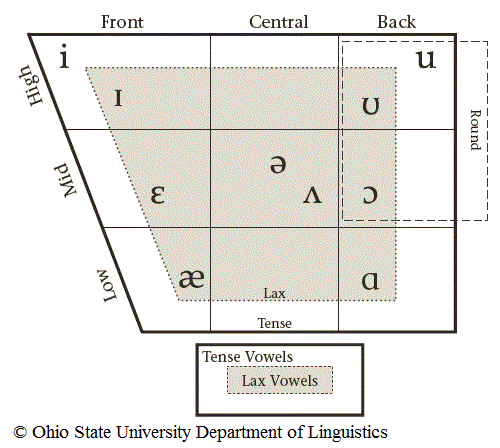
\includegraphics[width=1.0\textwidth]{img/English-monophthongs.png}\\
            단모음
        \end{column}
        \begin{column}{0.47\textwidth}
            \centering
            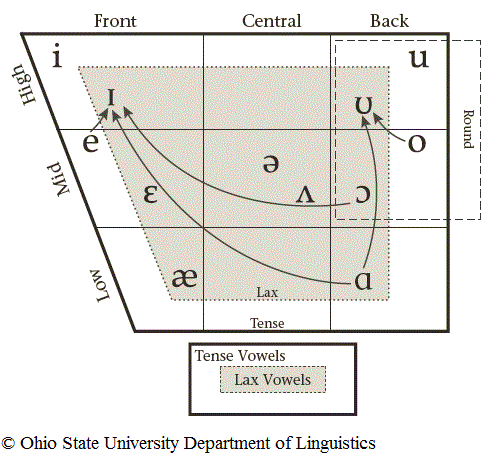
\includegraphics[width=1.0\textwidth]{img/English-diphthongs.png}\\
            이중모음            
        \end{column}
    \end{columns}

\end{frame}

\begin{frame}[t]{Abkhaz어의 음소}
    자음 58개: \\
    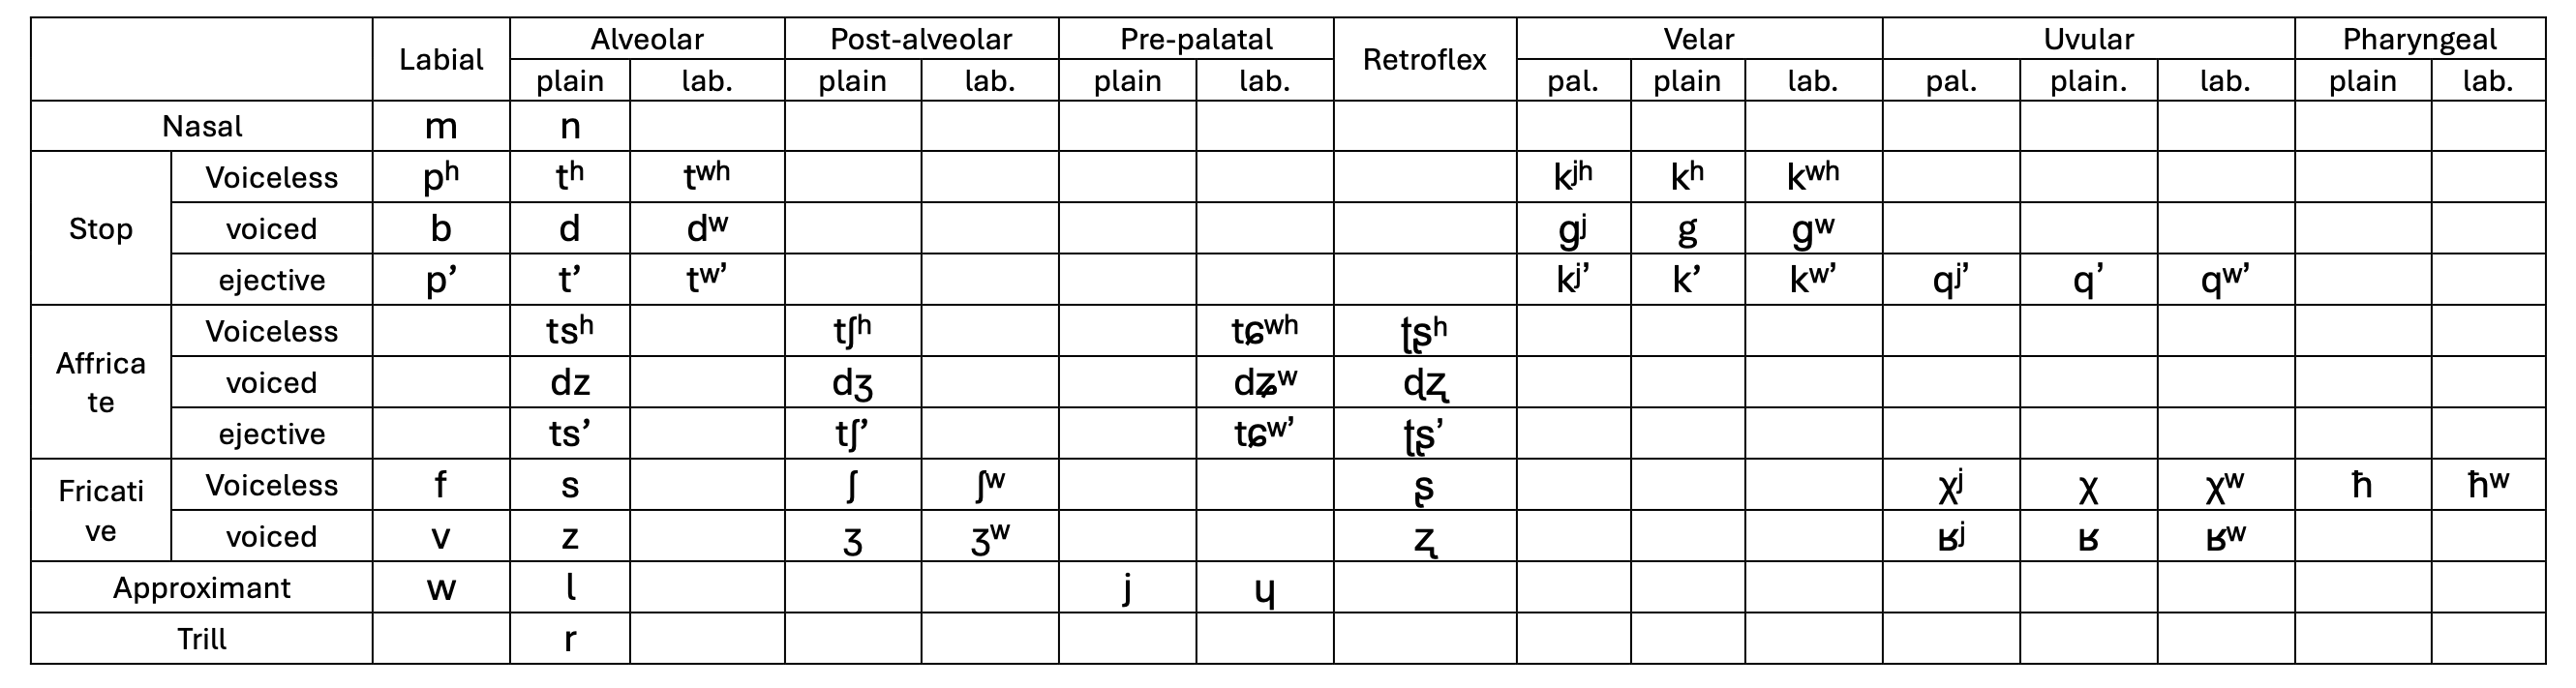
\includegraphics[width=1.0\textwidth]{img/Abkhaz_consonant_chart.png}\\
    모음 2개: \\
    고모음, 저모음
\end{frame}

\section{음운 규칙}

\begin{frame}[t]{음운 규칙(phonological rules)}
    \begin{block}{음운 규칙의 예: 변이음 규칙}
        \begin{itemize}
            \item 음소 : 변이음은 1 : 多 관계
            \item 변이음마다 출현하는 환경이 정해져 있음
            \item 음소 \rightarrow 환경에 따라 변이음 선택 \rightarrow 음성 발화
        \end{itemize}        
    \end{block}
    \begin{block}{미국 영어 \textds{/t/}}
        \begin{itemize}
            \item seat \textds{[sit]}, loot \textds{[lut]} \leftarrow 그 외 환경에서 변이음 \textds{[t]}로 실현
            \item seated \textds{[siɾəd]}, looted \textds{[luɾəd]} \leftarrow 강세 모음과 비강세 모음 사이에서 변이음 \textds{[ɾ]}로 실현
            \item tough \textds{[tʰʌf]} \leftarrow 어두에서 변이음 \textds{[tʰ]}로 실현
            \item written \textds{[rɪʔn̩]} \leftarrow 성절음 \textds{[n̩]} 앞에서 변이음 \textds{[ʔ]}으로 실현
        \end{itemize}
    \end{block}
    “\textasciitilde 한 환경에서” : 음운 규칙의 적용 환경(conditioning environment)
\end{frame}

\begin{frame}[t]{음운 규칙(phonological rules)}
    \begin{columns}
        \begin{column}[t]{0.46\textwidth}
            \begin{block}{음운 규칙의 일반화}
                X \rightarrow Y / C \_\_\ D 
            \end{block}            
        \end{column}
        \begin{column}[t]{0.47\textwidth}
            \begin{itemize}
                \item X는
                \item C와 D 사이에서
                \item Y로 실현된다
            \end{itemize}            
        \end{column}
    \end{columns}
    \begin{block}{미국 영어 \textds{/t/}의 변이음 규칙}
        \begin{itemize}
            \item \textds{/t/} \rightarrow \textds{[ɾ]} / 강세 모음 \_\_ 비강세 모음
            \item \textds{/t/} \rightarrow \textds{[tʰ]} / \# \_\_ 
            \item \textds{/t/} \rightarrow \textds{[ʔ]} / \_\_ \{\#, \textds{[n̩]}\}
            \item \textds{/t/} \rightarrow \textds{[t]} / 그 외
        \end{itemize}
    \end{block}
    \# : 단어 경계
\end{frame}

\begin{frame}[t]{자연 부류(natural classes)}
    \begin{columns}
        \begin{column}{0.46\textwidth}
            \begin{block}{미국 영어 \textds{/t/}의 변이음 규칙}
                \begin{itemize}
                    \item \textds{/t/} \rightarrow \textds{[ɾ]} / 강세 모음 \_\_ 비강세 모음
                    \item [] seat \textds{[sit]}
                    \item [] seated \textds{[siɾəd]}
                \end{itemize}
            \end{block}            
            \begin{block}{{미국 영어 \textds{/t/}, \textds{/d/}의 기술}}
                \textds{/t/}: 치경음, 파열음, 무성음\\
                \textds{/d/}: 치경음, 파열음, 유성음
            \end{block}            
        \end{column}
        \begin{column}{0.47\textwidth}
            \begin{block}{미국 영어 \textds{/d/}의 변이음 규칙}
                \begin{itemize}
                    \item \textds{/d/} \rightarrow \textds{[ɾ]} / 강세 모음 \_\_ 비강세 모음
                    \item [] seed \textds{[sid]}
                    \item [] seeded \textds{[siɾəd]}
                \end{itemize}
            \end{block}            
            \begin{block}{치경파열음}
                /t/와 /d/를 묶어서 한번에 골라낼 수 있는 자연 부류
            \end{block}
        \end{column}
    \end{columns}
    \begin{block}{\textds{[ɾ]} 변이음 관련 규칙의 재기술}
        치경파열음 \rightarrow \textds{[ɾ]} / 강세 모음 \_\_ 비강세 모음
    \end{block}            
\end{frame}

\begin{frame}[t]{자연 부류(natural classes)}
    \begin{block}{자연 부류}
        개별 언어의 말소리 중에서, 조음적 특성 또는 음향적 특성을 공유하는 소리들의 묶음
    \end{block}
    \begin{block}{자연부류의 예: 미국 영어}
        \begin{itemize}
            \item 긴장모음(tense vowel): \textds{[i], [u], [eɪ], [oʊ]}
            \item 연구개음(velar consonants): \textds{[k], [g], [ŋ]}
            \item 치찰음(sibilants): \textds{[s], [ʃ], [tʃ], [z], [ʒ], [dʒ]}
            \item 순음(labial): \textds{[p], [b], [m], [w], [f], [v]}
            \item 양순음(bilabial): \textds{[p], [b], [m]}
        \end{itemize}
    \end{block}
\end{frame}

\begin{frame}[t]{자연 부류(natural classes): 연습}
    다음은 미국 영어에 존재하는 모든 자음입니다. 이 목록 안에서 다음의 자연 부류를 찾아내 보세요! \\
    {\textds{/p/, /t/, /k/, /b/, /d/, /g/, /f/, /v/, /θ/, /ð/, /s/, /z/, /ʃ/, /ʒ/, /h/, /tʃ/, /dʒ/, /m/, /n/, /ŋ/, /l/, /ɹ/, /w/, /j/}}
    \vspace{0.3cm}
    \begin{itemize}
        \item 비음(nasals): {\small 조음 과정에서 비강이 열려 있는 소리} % 비음 /m, n, ŋ/
        \item 유음(liquid): {\small 공기의 흐름을 거의 방해하지 않으면서 혀의 모양이나 위치를 조정해서 만들어지는 소리} % 유음 /l/, /ɹ/
        \item 활음(glide): {\small 고모음과 거의 유사하게 조음되는데 다른 모음에 결합해서만 실현되는 소리} % 활음 /j/, /w/
        \item 공명음(sonorants): {\small 조음 과정에서 비강이 열려 있거나 구강이 상대적으로 열려 있는 소리} % 비음, 유음, 활음
        \item 장애음(obstruents): {\small 조음 과정에서 비강이 닫혀 있고 구강에서 공기의 흐름이 심하게 방해받는 소리} %파열음, 마찰음, 파찰음
    \end{itemize}
\end{frame}

\begin{frame}[t]{자연 부류(natural classes): 연습}
    다음은 한국어에 존재하는 모든 자음입니다. 이 목록 안에서 다음의 자연 부류를 찾아내 보세요! \\
    {\textds{/p/, /t/, /k/, /pʰ/, /tʰ/, /kʰ/, /p\textsuperscript{*}/, /t\textsuperscript{*}/, /k\textsuperscript{*}/, /s/, /s\textsuperscript{*}/, /h/, /tɕ/, /tɕʰ/, /tɕ\textsuperscript{*}/, /m/, /n/, /ŋ/, /l/, /w/, /j/}}
    \vspace{0.3cm}
    \begin{itemize}
        \item 비음(nasals) % 비음 /m, n, ŋ/
        \item 유음(liquid) % 유음 /l/
        \item 활음(glide) % 활음 /j/, /w/
        \item 공명음(sonorants) % 비음, 유음, 활음
        \item 장애음(obstruents) %파열음, 마찰음, 파찰음
    \end{itemize}
    \vspace{0.3cm}
    {\small 주의: 한국어의 /w/, /j/는 연구자에 따라 자음 대신 따로 반모음으로 분류하기도 합니다.}
\end{frame}

\begin{frame}[t]{음운 규칙의 종류}
    \begin{block}{동화(assimilation): 한국어 비음 동화}
        \begin{itemize}
            \item 한국어 \textds{/p/} \rightarrow \textds{[m]} / \_\_ \textds{\{[m], [n]\}} 밥물 \textds{[pammul]}, 겁나 \textds{[kʌmnɑ]}
            \item 한국어 \textds{/t/} \rightarrow \textds{[n]} / \_\_ \textds{\{[m], [n]\}} 맏물 \textds{[mɑnmul]}, 믿는 \textds{[minnɯn]}
            \item 한국어 \textds{/k/} \rightarrow \textds{[ŋ]} / \_\_ \textds{\{[m], [n]\}} 국물 \textds{[kuŋmul]}, 국내 \textds{[kuŋnæ]}
        \end{itemize}
    \end{block}
    \begin{block}{{자연부류를 이용한 한국어 비음 동화의 기술 : 파열음 \rightarrow 비음 / \_\_ 비음}}
        \begin{tabular}{llll}
            \textds{[p]} & 파열음, 양순음 & \textds{[m]} & 비음, 양순음 \\
            \textds{[t]} & 파열음, 치조음 & \textds{[n]} & 비음, 치조음 \\
            \textds{[k]} & 파열음, 연구개음 & \textds{[ŋ]} & 비음, 연구개음 \\
        \end{tabular}        
    \end{block}
\end{frame}

\begin{frame}[t]{음운 규칙의 종류}
    \begin{block}{동화(assimilation): 영어 구개음화}
        \begin{itemize}
            \item Did you? \textds{[dɪd.ju]} \textasciitilde \textds{[dɪdʒu]}
            \item [] 치경파열음 \textds{[d]}가 경구개접근음 \textds{[j]} 앞에서 경구개 쪽으로 조음점이 당겨지며 후치경파찰음 \textds{[dʒ]}로 발음됨
        \end{itemize}
    \end{block}
    \begin{block}{동화(assimilation): 핀란드어 모음조화(vowel harmony)}
        \begin{itemize}
            \item ‘house’ \textds{[tɑlo]} + 접사 ‘in’ : \textds{[tɑlo-ssɑ]}
            \item ‘forest’ \textds{[metsæ]} + 접사 ‘in’ : \textds{[metsæ-ssæ]}
            \item [] 같은 단어 안에서 후행 모음은 전설성/후설성이 선행 모음과 동일하게 바뀜
            \item [] 같은 단어 내의 모음은 모두 전설이거나 모두 후설
        \end{itemize}
    \end{block}
    원순성, 전설성/후설성 등 여러 자질을 토대로 모음조화가 발생할 수 있음
\end{frame}

\begin{frame}[t]{음운 규칙의 종류}
    \begin{block}{이화(dissimilation): 그리스어 조음방법 이화}
        \begin{itemize}
            \item ‘seven’ \textds{/epta/} \rightarrow \textds{[efta]}
            \item ‘building’ \textds{/ktizma/} \rightarrow \textds{[xtizma]}
            \item [] 파열음이 인접하면 선행하는 파열음이 마찰음으로 변화하는 현상
        \end{itemize}
    \end{block}
    이화가 일어나면 인접한 두 소리가 어떤 식으로든 서로 더 달라짐
    \begin{block}{삽입(insertion): 영어 무성파열음 삽입}
        \begin{itemize}
            \item strength \textds{/stɹɛŋθ/} \rightarrow \textds{[stɹɛŋkθ]}
            \item hamster \textds{/hæmstɹ̩/} \rightarrow \textds{[hæmpstɹ̩]}
            \item [] 무성마찰음과 비음 사이에 비음과 조음위치가 동일한 무성파열음이 삽입되는 현상
        \end{itemize}
    \end{block}
\end{frame}

\begin{frame}[t]{음운 규칙의 종류}
    \begin{block}{탈락(deletion): 한국어 \textds{/h/} 탈락}
        \begin{itemize}
            \item 좋으니 \textds{[tɕo.ɯ.ni]} (참고: 좋고 \textds{[tɕo.kʰo]})
            \item 전화 \textds{[tɕʌn.hwɑ]} \textasciitilde \textds{[tɕʌ.nwɑ]}
            \item [] 모음 앞에서 \textds{/h/}가 탈락하는 현상
        \end{itemize}
    \end{block}
    \begin{block}{전위(metathesis): Leti 어 자음군 전위}
        VCCC \rightarrow CVCC 
        \begin{itemize}
            \item ‘집게손가락’ \textds{/ukar + ppalu/} \rightarrow \textds{[ukrappalu]}
            \item ‘노래기’ \textds{/danat + kviali/} \rightarrow \textds{[dantakviali]}
        \end{itemize}
    \end{block}
    cf. VCCV : 전위 없음
    \begin{itemize}
        \item ‘엄지손가락’ \textds{/ukar + lavan/} \rightarrow \textds{[ukarlavan]}
    \end{itemize}
\end{frame}

\begin{frame}[t]{음운 규칙의 종류}
    \begin{block}{강화(strengthening): 영어 무성파열음의 유기음화}
        \begin{itemize}
            \item 무성파열음 \rightarrow 무성유기파열음 / \# \_\_
            \item [] {\small 무성유기파열음은 무성파열음보다 무성 구간이 더 긺 \rightarrow 더 ‘강한’ 자음으로 분류}
        \end{itemize}
    \end{block}    
    \begin{block}{약화(weakening): 영어 치경파열음의 탄설음화}
        \begin{itemize}
            \item 치경파열음 \rightarrow 탄설음 / 강세 모음 \_\_ 비강세 모음
            \item [] {\small 탄설음은 파열음보다 더 짧게 실현되고 공기의 흐름을 덜 방해 \rightarrow 더 ‘약한’ 자음으로 분류}
        \end{itemize}
    \end{block}
    \begin{block}{약화(weakening): 영어 비강세모음 축약}
        \begin{itemize}
            \item atom \textds{/ˈætəm/} \rightarrow \textds{[ˈæɾm̩]} 
            \item [] {\small 비강세모음이 \textds{[ə]}가 되거나 뒤따르는 자음을 성절성 자음으로 바꾸고 사라짐}
        \end{itemize}
    \end{block}
\end{frame}

\begin{frame}[t]{음운 규칙의 다중 적용}
    \begin{block}{규칙의 적용 순서를 알 수 없는 경우}
        \begin{columns}
            \begin{column}{0.46\textwidth}
                \begin{center}
                    탄설음화가 모음축약에 선행
                \end{center}
                \begin{tabular}{ll}
                    & photograph \\
                    음소형 & \textds{/ˈfoʊtoʊgɹæf/} \\
                    탄설음화 & \textds{ˈfoʊɾoʊˌgɹæf}\\
                    모음 축약 & \textds{ˈfoʊɾəˌgɹæf}\\
                    음성형 & \textds{[ˈfoʊɾəˌgɹæf]}                    
                \end{tabular}
            \end{column}
            \begin{column}{0.47\textwidth}
                \begin{center}
                    모음축약이 탄설음화에 선행
                \end{center}
                \begin{tabular}{ll}
                    & photograph \\
                    음소형 & \textds{/ˈfoʊtoʊgɹæf/} \\
                    모음 축약 & \textds{ˈfoʊtəˌgɹæf}\\
                    탄설음화 & \textds{ˈfoʊɾəˌgɹæf}\\
                    음성형 & \textds{[ˈfoʊɾəˌgɹæf]}
                \end{tabular}
            \end{column}
        \end{columns}
    \end{block}
    \begin{itemize}
        \item 탄설음화와 모음 축약 중 어느 것이 먼저 일어나도 최종 음성형은 동일함
        \item 따라서 어느 규칙이 먼저인지 이 데이터로는 알 수 없음
    \end{itemize}
\end{frame}

\begin{frame}[t]{음운 규칙의 다중 적용}
    \begin{block}{규칙의 적용 순서가 분명한 경우}
        미국영어 방언의 이중모음화: 무성음 앞에서 이중모음 \textds{/ɑɪ/}가 \textds{[ʌɪ]}로 상승
        \begin{columns}
            \begin{column}{0.46\textwidth}
                \begin{center}
                    탄설음화가 이중모음 상승에 선행
                \end{center}
                \begin{tabular}{ll}
                    & writer\\
                    음소형 & \textds{/ˌɹɑɪtəɹ/} \\
                    탄설음화 & \textds{ˌɹɑɪɾəɹ}\\
                    이중모음 상승 & -- \\
                    음성형 & *\textds{[ˌɹɑɪɾɹ̩]}
                \end{tabular}
            \end{column}
            \begin{column}{0.47\textwidth}
                \begin{center}
                    이중모음 상승이 탄설음화에 선행
                \end{center}
                \begin{tabular}{ll}
                    & writer\\
                    음소형 & \textds{/ˌɹɑɪtəɹ/}\\
                    이중모음 상승 & \textds{ˌɹʌɪtəɹ}\\
                    탄설음화 & \textds{ˌɹʌɪɾəɹ}\\
                    음성형 & \textds{[ˌɹʌɪɾɹ̩]}
                \end{tabular}
            \end{column}
        \end{columns}        
    \end{block}
    \begin{itemize}
        \item 이 방언에서는 rider \textds{[ˌɹɑɪɾɹ̩]}와 writer \textds{[ˌɹʌɪɾɹ̩]}를 구분함
        \item 따라서 이중모음 상승 > 탄설음화가 올바른 순서
    \end{itemize}
\end{frame}

\begin{frame}[t]{의무적 음운규칙과 수의적 음운규칙}
    \begin{block}{의무적 음운규칙(obligatory rules)}
        환경이 갖춰지면 반드시 적용되는 규칙
        \begin{itemize}
            \item 한국어 모음어미 앞에서 용언의 /h/ 말음 탈락 (‘좋으니’)
            \item Leti 어 자음군 전위
            \item 한국어 비음 동화
            \item 영어 탄설음화
        \end{itemize}
    \end{block}
    이른바 ‘외국식 악센트’의 발생 원인: 모어의 의무적 음운 규칙을 외국어에 적용하는 경우
    \begin{block}{수의적 음운규칙(optional rules)}
        환경이 갖춰져도 일어나지 않을 수 있는 규칙
        \begin{itemize}
            \item 한국어 명사에서의 /h/ 탈락 (‘전화’)
        \end{itemize}
    \end{block}
\end{frame}

\section{음소 체계의 보편적 경향}

\begin{frame}[t]{흔한 소리와 덜 흔한 소리}
    \begin{block}{모든 말소리가 고르게 나타나는 것은 아님}
        \begin{itemize}
            \item \textds{[p], [t], [a]}: 아주 많은 언어에서 확인됨
            \item 인두음, 흡착음, 무성 모음 등: 소수의 언어에서 확인됨
        \end{itemize}
    \end{block}
    \begin{block}{음소의 ‘흔함’을 토대로 음소 출현 예측하기}
        \begin{itemize}
            \item 흔하지 않은 말소리가 존재한다면 그것의 흔한 짝도 존재할 것
            \item [] 무성 모음이 쓰이는 언어라면 유성 모음도 쓰일 것
            \item [] 무성 인두 마찰음이 쓰이는 언어라면 무성 연구개 마찰음도 쓰일 것
            \item 무성 연구개 마찰음을 쓰면서 무성 치경 마찰음을 안 쓰는 언어는 상상하기 어려움
        \end{itemize}
    \end{block}
\end{frame}

\begin{frame}[t]{흔한 소리와 덜 흔한 소리}
    \begin{block}{‘흔함’ 기준으로 짝이 되는 소리들}
        \begin{tabular}{ll}
            \hline
            \textbf{덜 흔함} & \textbf{더 흔함}\\
            \hline
            \textds{[ã]} & \textds{[a]} \\
            \textds{[ḁ]} & \textds{[a]} \\
            \textds{[x]} & \textds{[k]} 또는 \textds{[s]} \\
            \textds{[s]} & \textds{[t]} \\
            \textds{[d]} & \textds{[t]} \\
            \textds{[ð]} & \textds{[d]} 또는 \textds{[z]} \\
            유성 파열음 & 무성 파열음 \\
            특정 조음 위치의 마찰음 & 같은 조음 위치의 파열음 \\
            \hline
        \end{tabular}
    \end{block}    
\end{frame}

\begin{frame}[t]{말소리의 ‘흔함’과 빈도/분포}
    \begin{block}{말소리의 ‘흔함’과 빈도}
        \begin{itemize}
            \item 흔하지 않은 말소리는 개별 언어에 쓰이더라도 덜 쓰임
            \item [] 영어의 \textds{[ð]}는 \textds{[z]}보다 출현 단어 수가 더 적음
        \end{itemize}
    \end{block}
    \begin{block}{말소리의 ‘흔함’과 분포}
        \begin{itemize}
            \item 흔하지 않은 말소리는 개별 언어에 쓰이더라도 출현이 제약됨
            \item [] 광동어의 마찰음은 어두에서만 출현 vs. 파열음은 어두와 어말 모두 출현
            \item [] 한국어의 경음, 유기음, 마찰음, 파찰음은 어말에 출현하지 못함(음절 끝소리 규칙)
        \end{itemize}
    \end{block}
\end{frame}

\begin{frame}[t]{말소리의 ‘흔함’과 습득/유지}
    \begin{block}{더 ‘흔한’ 소리가 더 ‘쉬움’}
        \begin{itemize}
            \item 제1언어 습득시 더 흔한 소리가 더 먼저 습득됨
            \item 아직 습득하지 못한 소리는 짝이 되는 더 흔한 소리로 대체하여 발음
            \item [] this one \textds{[dɪs wʌn]} (\textds{[d]} vs. \textds{[ð]})
        \end{itemize}
    \end{block}
    \begin{block}{더 ‘흔한’ 소리가 더 ‘잘 버팀’}
        \begin{itemize}
            \item 더 드문 소리는 언어 변화로 없어질 가능성이 더 큼
            \item [] 고대영어 \textds{[x]}의 소실 (묵음 철자 ‘gh’)
            \item [] \rightarrow knight, height, sight, fight, might ... 
            \item [] \textds{[k]}가 안정적으로 유지되고 있는 것과 대비되는 변화
        \end{itemize}
    \end{block}
\end{frame}

\begin{frame}[t]{음소 체계의 보편성은 왜 존재하는가}
    \begin{block}{조음의 편의성}
        \begin{itemize}
            \item 발음하기 어려운 말소리는 조음이 일관적이지 않거나 실패할 가능성이 상대적으로 큼
            \item 화자들이 되도록 사용을 피함
            \item 어린 화자는 습득하기 어려움
        \end{itemize}
    \end{block}
    \begin{block}{청취의 편의성}
        \begin{itemize}
            \item 자음과 모음의 조합으로 말소리의 한 단위가 구성됨
            \item 구성요소들이 잘 구분될수록 단위를 파악하기도 쉬워짐
            \item [] \rightarrow 모음 같지 않은 자음과 자음 같지 않은 모음을 선호하는 경향
            \item [] \textds{[i], [u]}가 있다면 \textds{[a]}의 존재를 예측 가능
        \end{itemize}
    \end{block}
\end{frame}

\section{음소 분석}

\begin{frame}[t]{음소 분석의 실제}
    미국 영어 \textds{[ɹ̥]} vs. \textds{[ɹ]}
    \begin{columns}
        \begin{column}[T]{0.33\textwidth}
            \begin{block}{전체 데이터 패턴}
                \begin{tabular}{ll}
                    pray & \textds{[pʰɹ̥eɪ]} \\
                    gray & \textds{[gɹeɪ]} \\
                    crab & \textds{[kʰɹ̥æb]} \\
                    par & \textds{[pʰɑɹ]} \\
                    broker & \textds{[bɹoʊkɹ̩]}\\
                    fresh & \textds{[fɹ̥ɛʃ]}\\
                    regain & \textds{[ɹiɡeɪn]}\\
                    shriek & \textds{[ʃɹ̥ik]}\\
                    tar & \textds{[tʰɑɹ]}
                \end{tabular}
            \end{block}            
        \end{column}
        \begin{column}[T]{0.3\textwidth}
            \begin{block}{\textds{[ɹ̥]}의 출현 환경}
                \begin{itemize}
                    \item \textds{[pʰ\_\_eɪ]}
                    \item \textds{[kʰ\_\_æb]}
                    \item \textds{[f\_\_ɛʃ]}
                    \item \textds{[ʃ\_\_ik]}
                \end{itemize}
            \end{block}
            \textds{[pʰ]}, \textds{[kʰ]}, \textds{[f]}, \textds{[ʃ]}의 공통점은?
        \end{column}
        \begin{column}[T]{0.3\textwidth}
            \begin{block}{\textds{[ɹ]}의 출현 환경}
                \begin{itemize}
                    \item \textds{[g\_\_eɪ]}
                    \item \textds{[pʰɑ\_\_]}
                    \item \textds{[b\_\_oʊkɹ̩]}
                    \item \textds{[\_\_iɡeɪn]}
                    \item \textds{[tʰɑ\_\_]}
                \end{itemize}
            \end{block}
            이 환경들을 단 하나의 기준으로 포착한다면?
        \end{column}
    \end{columns}
\end{frame}

\begin{frame}[t]{음소 분석의 실제}
    \begin{columns}
        \begin{column}[T]{0.46\textwidth}
            \begin{enumerate}
                \item 서로 다른 음성 포착
                \item 각각의 음성이 출현하는 모든 환경 포착
                \item 같은 환경에서 출현하는 다른 소리가 있는지 확인
                    \begin{itemize}
                        \item 최소대립쌍이 성립하는지 확인
                            \begin{itemize}
                                \item 성립하면 음소
                                \item 성립하지 않으면 자유변이
                            \end{itemize}
                    \end{itemize}
                \item 같은 환경에서 출현하는 다른 소리가 없다면 상보적 분포가 성립하는지 확인
                \item 상보적 분포를 이루는 쌍이 있으면 변이음 규칙을 쓸 수 있는지 확인
            \end{enumerate}            
        \end{column}
        \begin{column}[T]{0.47\textwidth}
            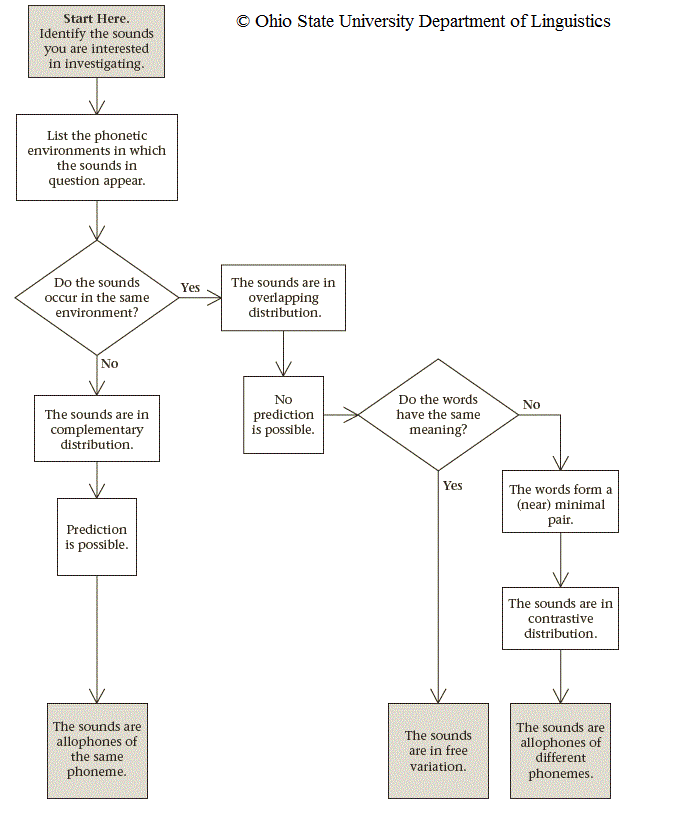
\includegraphics[width=0.9\textwidth]{img/phonology-flowchart.png}
        \end{column}
    \end{columns}
\end{frame}

\begin{frame}[t]{음소 분석의 실제}
    우크라이나어 \textds{[s], [sʲ], [ʃ], [ʃʲ]}\\
    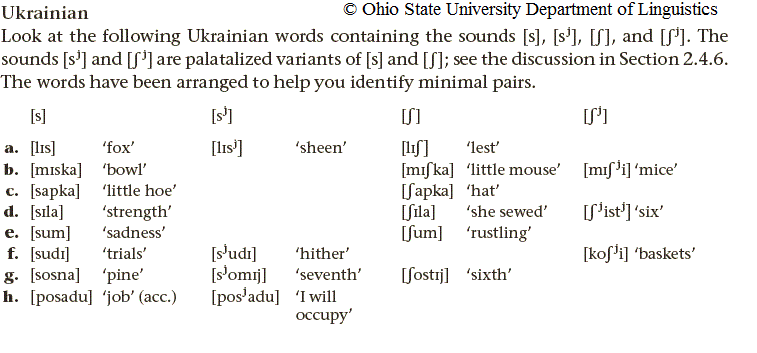
\includegraphics[width=1.0\textwidth]{img/exer9-Ukrainian-data.png}
\end{frame}

\begin{frame}[t]{음소 분석의 실제}
    우크라이나어 \textds{[s], [sʲ], [ʃ], [ʃʲ]}\\
    \begin{itemize}
        \item 최소대립쌍을 있는 대로 찾아내세요.
        \item 3개로 이루어진 최소대립쌍도 있나요? 찾아보세요.
        \item 이 4개의 말소리 가운데 대립성이 있는 소리들은 무엇인가요?
        \item 4개의 말소리 중 1개는 특정한 모음 앞에서만 출현합니다. 무엇이 어느 모음 앞에서 나타나나요?
    \end{itemize}
\end{frame}

\begin{frame}[t]{참고문헌}
  \begin{itemize}
    \item \texttnr{Department of Linguistics, The Ohio State University (2022) \textit{Language Files}, 13th ed. Ohio State University Press. Chapter 3.}
    \item 신지영 (2022) 《말소리의 이해》, 2판. 한국문화사
  \end{itemize}    
\end{frame}


\end{document}